% !TeX root = ../main.tex

%%%%%%%%%%%%%%%%%%%%%%%%%%%%%%%%%%%%%%%%%%%%%%%%%%%%%%%%%%%%%%%%%%%%%%%%%%%%%%%%%%
%%																				%%
%% File name: 		body.tex													%%
%% Project name:	Applications in Deep Learning								%%
%% Type of work:	Advanced Seminar											%%
%% Author:			Hannes Bohnengel											%%
%% Mentor:			Debayan Roy													%%
%% Date:			05 June 2017												%%
%% University:		Technical University of Munich								%%
%% Comments:		Created in texstudio with tab width = 4						%%
%%																				%%
%%%%%%%%%%%%%%%%%%%%%%%%%%%%%%%%%%%%%%%%%%%%%%%%%%%%%%%%%%%%%%%%%%%%%%%%%%%%%%%%%%

\section{Conventional Speech Synthesis}
\label{sec:speech}

\subsection{Motivation \& Approaches}
\label{subsec:convenspeech}

Speech synthesis has emerged over the last 10 years due to a vast contribution by the global community of researchers and the increasing computational power for data processing. Its quality and naturalness has increased steadily and different approaches have been developed so far \cite{suendermann:challenges}. The typical applications like navigation systems in cars or telephone-based dialogue systems are nowadays widely established. But also as reading aid for visually impaired people \cite{readspeaker:tts} or as in the case of the famous scientist Stephen Hawking, who has been using a synthesized voice to communicate since 1997 \cite{hawking:speech}, speech synthesis has proven to be very useful. Another very interesting application of speech synthesis is shown in [XX]. The author proposed to introduce synthetic speech as means of communication between pilots, since there have been many accidents due to missunderstandings at radio-based communication. %Finally the interaction between man and machines or robots \cite{hill:manmachine}

According to \cite{hinterleitner:quality} speech synthesis can be divided into three types: Canned speech, \ac{CTS} and \ac{TTS}. Canned speech more or less is the replay of prerecorded spoken sentences or words with none or very little adjustments. A typical example are the announcements on train stations. Because of the high effort of recording everything (almost) exactly as it is replayed, this approach is limited to only a few simple applications. With \ac{CTS} the waveform is generated out of a linguistic description without any information of the respective text. In this way no natural language processing is required, but nevertheless \ac{CTS} nowadays has not made any important impact. The last and most promising type is \ac{TTS}.

A \ac{TTS} system consists of a \ac{NLP} part, where the text is analysed and the word and sentence structure and accents are extracted. In the next step these accents are used to generate the prosody of the given text like duration, intensity and pitch. Then the created phonetic represantations with prosody information are stringed together to a continuous stream of signal parameters. The last task, the speech generation, uses this stream to generate the respective waveform. This function block can be implemented in different ways. In \cite{hinterleitner:quality} three general approaches are named as follows: Parametric Speech Synthesis (formant-based synthesis), Concatenative Speech Synthesis (unit-selection synthesis) and Statistical Parametric Speech Synthesis (\ac{HMM}-based synthesis). The methods in brackets are the respective implementations, which are most commonly used. 

The formant-based synthesis is the oldest approach. To generate a voice waveform, an excitation signal is fed into multiple formant filters which describe the characteristics of the human vocal tract. The output of the filters then forms the voice waveform. This technique is the only one which does not need any recorded speech, but instead generates the synthesized voice only by modeling the human vocal tract. The quality of the generated voice is the lowest in comparison to the other techniques, but therefore formant-based synthesizer have the smallest footprint and the voice characteristics can easilily been modified by just changing the filter parameters~\cite{hinterleitner:quality}.

With the development of concatenative speech synthesizer the quality of the generated speech improved tremendously. Very similar to \ac{CTS} prerecorded speech is used as reference. Very basically said, the recorded speech is devided into units and these units are then stringed together to form the new speech signal according to a given text. Hereby the chosen size of the units determines both the footprint size and the voice quality. With larger units a higher voice quality can be achieved, but this also results in a much larger database. The challenge in unit-selection is to ensure, that the transissions between the units are as natural as possible~\cite{hinterleitner:quality}. In Section~\ref{subsec:hmmspeech} some concepts on how to achieve this as well as the third implementation, the \ac{HMM}-based synthesis, a specific instance of \ac{SPSS} are described in detail.

\subsection{\ac{HMM}-based Speech Synthesis}
\label{subsec:hmmspeech}

In this section the \ac{HMM}-based, the most recent approach for speech synthesis will be described further and both advantages and drawbacks compared to unit-selection synthesis will be highlighted. Therefore the work of Zen et al. \cite{zen:statistical} will be taken as reference.

The quality of unit-selection synthesis directly depends from the quality of the prerecorded speech. But even with a database of excellent quality sporadic errors can still not be avoided totally. If a specific phonetic or prosodic part of a generated sentence is not well represented in the database the output quality of this sentence suffers immensely. To try to avoid this a huge effort in specifically designing the database for the required application can be performed, but still there is no guarantee that such bad joins happen. In addition the fact, that in unit-selection no or only very little adaptions of the voice characteristics are possible without an enormous increase of the database size, the ambition towards seamless speech synthesis leads to the \ac{HMM}-based approach. There a statistic representation of some sets of speech segments is used to generate arbitrary synthetic speech.

\textbf{{\color{ACMRed}Details about unit-selection synthesis ???}}

In Figure~\ref{fig:hmm} the structure of a typical \ac{HMM}-based synthesizer is shown. The whole system can be devided into two parts, the training and the synthesis part. The connection of these two parts are a number of context-dependent ({\color{ACMRed}what is that?}) \acp{HMM}. In the training part spectrum and excitation parameters of the recorded speech are used to generate acoustic models represented by the \acp{HMM}. Thereby phonetic, linguistic and prosodic parameters are considered. {\color{ACMRed}Details about spectrum and excitation parameters?} In comparison to a unit-selection system the database only is needed in the training part.

\begin{figure}[h]
	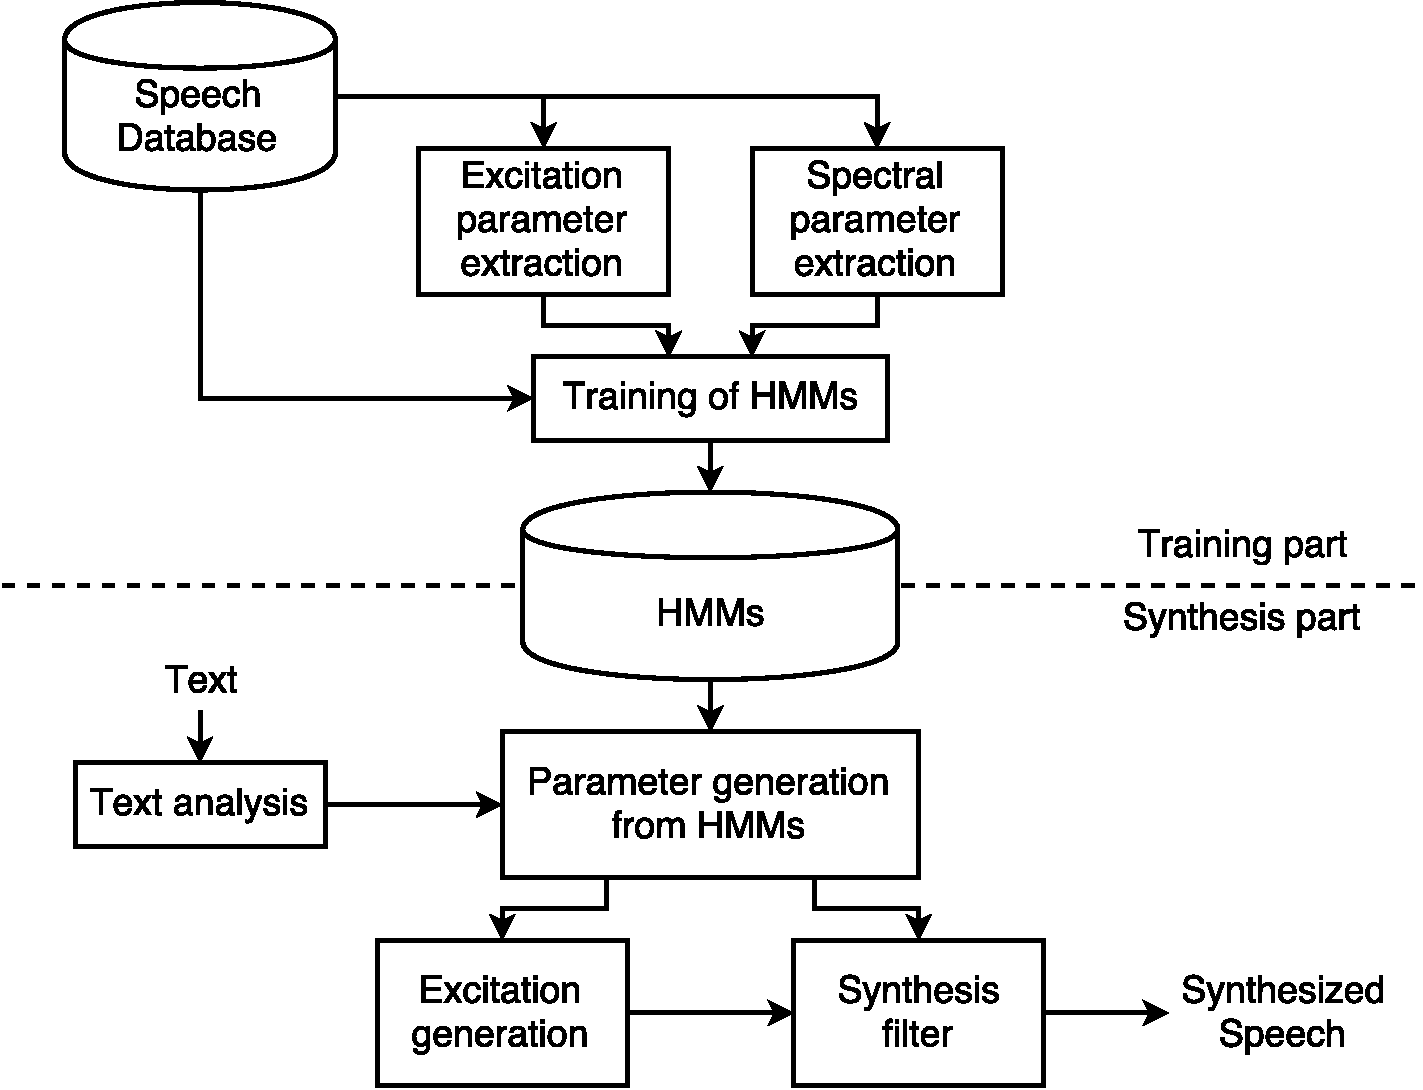
\includegraphics[width=0.8\columnwidth]{hmm-system.pdf}
	\caption{Function blocks of \ac{HMM}-based synthesis \cite{zen:statistical}}
	\label{fig:hmm}
\end{figure}

In the synthesis part first the text which is to be synthesized is 

\newpage

The main disadvantage of this approach compared to unit-selection synthesis is the quality of the synthesized speech. Three factors are accountable for the lack of quality: vocoder, modeling accuracy, and over-smoothing.

{\color{ACMRed}In Table~\ref{tab:speechgeneration} these techniques are compared regarding the most prominent advantages and drawbacks.}

\begin{table}[h]
	\caption{Comparison of speech generation methods~\cite{hinterleitner:quality, zen:statistical}}
	\label{tab:speechgeneration}
	\begin{tabularx}{1\columnwidth}{lYY}
		\toprule
		Technique & Advantages & Drawbacks\\
		\midrule
		Formant-based & No prerecorded speech required & Very artificial and metallic voice\\[0.5em]
		Unit-selection & Very high voice quality possible & Large database required\\[0.5em]
		\ac{HMM}-based & Adjustable voice and small footprint & Voice sounds muffled\\
		\bottomrule
	\end{tabularx}
\end{table}


\vspace{1em}\ \\
\textbf{Why there is need to further improve this technology?}\\
\textbf{What is a HMM?}

\clearpage


%---------------------------------------------------------------------------------
%---------------------------------------------------------------------------------
% SPSS with Deep Learning Models
%---------------------------------------------------------------------------------
%---------------------------------------------------------------------------------

\section{\ac{SPSS} with Deep Learning Models}
\label{sec:deepspeech}

\subsection{General ways for improvement}
\label{subsec:deepeffect}

In \cite{hashimoto:effect} the effects of deep learning methods on \ac{SPSS} are investigated. Therefore the different parts of a \ac{HMM}-based speech synthesis system are modeled with a \ac{DNN} and then the output is compared to the conventional approach.

\subsection{One specific approach for improvement}
\label{subsec:deepspss}

Statistical parametric speech synthesis using deep neural networks \cite{zen:deepstatistical}

%---------------------------------------------------------------------------------
%---------------------------------------------------------------------------------
% Speech Synthesis on Embedded Devices
%---------------------------------------------------------------------------------
%---------------------------------------------------------------------------------

\section{Speech Synthesis on Embedded Devices}
\label{sec:embeddedspeech}

\subsection{Motivation}
\label{subsec:motembedded}

Why is it important to implement speech synthesis on embedded platform?\\
What needs to be thought about when dealing with embedded or mobile devices?

\subsection{\ac{HMM}-based Approach}
\label{subsec:hmmembedded}

An example of how speech synthesis can be implemented on embedded platform without deep learning (core paper~3).

\subsection{Deep Learning-based Approach}
\label{subsec:deepembedded}

An example of how speech synthesis can be implemented on embedded platform WITH deep learning (core paper 4).

\clearpage
